%!TEX root = ../main.tex
%%%%%%%%%%%%%%%%%%%%%%%%%%%%%%%%%%
% Links:
%
% Difficulty: Companies: 
%%%%%%%%%%%%%%%%%%%%%%%%%%%%%%%%%%


%\begin{figure} \centering
%   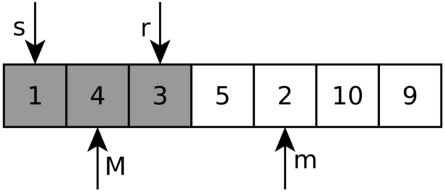
\includegraphics[width=\textwidth]{sources/max_num_chunks_sorted/images/example1}
%   \caption[Sample short cpation]{Sample Caption}. \label{fig:max_num_chunks_sorted:example1}
%   \end{figure}

\chapter{Sort the chunks, sort the array.}
\label{ch:max_num_chunks_sorted}
\section*{Introduction}

Sorting is a popular topic in computer science and in programming interview. Its usefulness its beyond dispute and 
is it not surprising that there are literally countless of research papers and algorithms on the topic. 

In this problem however we are not going to devise a novel sorting algorithm, instead 
we are going to investigate on a less useful problem,
that challenge us to find out how we can split an array into pieces such that if each of the pieces is sorted 
individually, the final result would be equivalent to having sorted the entire array to begin with.

It is necessary to develop a key insight to solve this problem efficiently, 
and asking the right questions and looking at a number of good examples
is fundamental for doing so. In the next section we are going to explore how these insight 
can be gained and then turned into an efficient code. 



\section{Problem statement}
\begin{exercise}
\label{example:max_num_chunks_sorted:exercice1}
Write a function that given an array $I$ of integers returns the maximum number of sub-arrays of $I$ 
such that if each of the subarray is sorted individually, then $I$ as a whole is sorted.

	%example1
	\begin{example}
		\label{example:max_num_chunks_sorted:example1}
		\hfill \\
		Given $I=\{45,88,1,9,90\}$ then the function return $1$.
		
	\end{example}

	%example2
	\begin{example}
		\label{example:max_num_chunks_sorted:example2}
		\hfill \\
		Given $I=\{4,3,2,1,5,9,10\}$ then the function return $4$. We can sort the following sub-arrays:
		\begin{itemize*}
			\item $[0,3]$
			\item $[4,4]$
			\item $[4,4]$
			\item $[4,4]$
		\end{itemize*}
	\end{example}
\end{exercise}

\section{Clarification Questions}

\begin{QandA}
	\item 
	\begin{answered}
		\textit{}
	\end{answered}
	
\end{QandA}

\section{Discussion}
\label{max_num_chunks_sorted:sec:discussion}


\subsection{Brute-force}
\label{max_num_chunks_sorted:sec:bruteforce}

\begin{minipage}{\linewidth}
	\lstinputlisting[language=c++, caption={Sample Caption},label=list:max_num_chunks_sorted]{sources/max_num_chunks_sorted/max_num_chunks_sorted_solution1.cpp}
\end{minipage}

